\documentclass[11pt,a4paper]{article}

\usepackage[T1]{fontenc}
\usepackage[utf8]{inputenc}
\usepackage{lmodern}
\usepackage{microtype}
\usepackage[a4paper,margin=2.6cm]{geometry}
\usepackage{amsmath,amssymb,mathtools}
\usepackage{booktabs}
\usepackage{array}
\usepackage{enumitem}
\usepackage{xcolor}
\usepackage{graphicx}
\usepackage{listings}
\usepackage{hyperref}
\usepackage{fancyhdr}
\usepackage{tikz}
\usetikzlibrary{arrows.meta,positioning}

\hypersetup{
    colorlinks=true,
    linkcolor=blue!45!black,
    urlcolor=blue!45!black,
    citecolor=blue!45!black,
    pdftitle={From Cayley Tables to Polyphony},
    pdfauthor={Orges Leka}
}

\pagestyle{fancy}
\setlength{\headheight}{14pt}
\fancyhf{}
\lhead{Orges Leka}
\rhead{From Cayley Tables to Polyphony}
\cfoot{\thepage}

\lstset{
    basicstyle=\ttfamily\small,
    frame=single,
    breaklines=true,
    columns=fullflexible,
    showstringspaces=false,
    backgroundcolor=\color{black!3}
}

\newcommand{\Z}{\mathbb{Z}}
\newcommand{\Sn}{S_n}
\newcommand{\modulo}[1]{\; (\mathrm{mod}\,#1)}

\title{\textbf{From Cayley Tables to Polyphony}\\[0.4em]
\large A Group-Theoretic Framework for Algorithmic Music Generation}
\author{Orges Leka\\[0.3em]\small Writing Assistant: ChatGPT}
\date{September 2026}

\begin{document}
\maketitle

\begin{abstract}
This paper describes an algorithmic composition method in which the multiplication structure of a finite group is transformed into polyphonic musical material. The central mechanism is the regular action of a finite group on itself: each group element acts by left multiplication and therefore induces a permutation of the underlying set. Rows of the Cayley table are interpreted as ordered traversal patterns, and these patterns are projected onto chord degrees by several voice-dependent maps. A second numerical process, obtained from the parity of decimal digits of a real constant, controls octave motion and rhythmic rotation. Dynamics are coupled to positions inside each group-induced permutation. The resulting system separates harmonic vocabulary from algebraic ordering: chord collections define the available pitch material, while the finite group controls how that material is traversed. The paper also analyzes an implementation detail of the parameter \texttt{iter\_it}, showing that in the present program it creates a redundant multiset expansion rather than an iterated group action and can cause systematic MIDI-velocity saturation. The construction provides a concrete example of how symmetry, permutation, and finite-state dynamics can be used as compositional principles.
\end{abstract}

\section{Introduction}

The compositional idea studied here is to use an abstract algebraic object not merely as a source of numbers, but as a source of \emph{structured transformations}. A finite group is particularly suitable for this purpose. Its multiplication law contains symmetry, reversibility, and a family of permutations that can be made audible.

Let
\[
G=\{g_0,g_1,\ldots,g_{n-1}\}
\]
be a finite group of order
\[
|G|=n.
\]
Instead of assigning one fixed pitch to each group element and reading the elements in an arbitrary order, the algorithm uses the regular action of $G$ on itself. For every $a\in G$, left multiplication
\[
L_a:G\longrightarrow G,\qquad x\longmapsto ax
\]
is a bijection. Hence each $a$ determines a permutation of the $n$ group elements. The group therefore generates an internally related family of orderings of the same finite set.

Musically, these orderings are interpreted as traversal patterns through harmonic material. The harmony is supplied independently as a list of chords. The group determines the order in which degrees of the current chord are selected, while additional finite-state processes determine register, duration, and dynamics.

The core conceptual pipeline is
\[
\boxed{
\text{group multiplication}
\longrightarrow
\text{permutation}
\longrightarrow
\text{index sequence}
\longrightarrow
\text{chord degree}
\longrightarrow
\text{pitch}
}.
\]
A second pipeline controls slower musical parameters:
\[
\boxed{
\text{digits of a real constant}
\longrightarrow
\{0,1\}\text{-sequence}
\longrightarrow
\text{register and rhythm states}
}.
\]

\section{The Regular Permutation Representation}

\subsection{Left and right regular actions}

For any fixed $a\in G$, the map
\[
L_a(x)=ax
\]
is bijective, with inverse $L_{a^{-1}}$. Therefore $L_a$ is a permutation of the underlying set of $G$. If the elements of $G$ are indexed by
\[
G=\{g_0,\ldots,g_{n-1}\},
\]
then $L_a$ becomes a permutation
\[
\sigma_a\in S_n.
\]
Moreover,
\[
L_a\circ L_b=L_{ab},
\]
so the map
\[
\rho_L:G\longrightarrow S_n,\qquad a\longmapsto \sigma_a
\]
is a group homomorphism. It is injective, because $L_a=L_b$ implies
\[
a=L_a(e)=L_b(e)=b.
\]
Thus every finite group is represented faithfully as a permutation group. This is the regular representation underlying the implementation.

The code also permits the right action
\[
R_a(x)=xa,
\]
although the musical generator itself uses products of the form $gh$, corresponding naturally to the left-regular viewpoint.

\subsection{From abstract elements to permutations}

The implementation enumerates the group elements, assigns them integer positions, and converts the images of the generators under left or right multiplication into permutations. If $\iota:G\to\{1,\ldots,n\}$ denotes the indexing function, then the permutation associated with $a$ is
\[
\sigma_a(i)=\iota\!\left(a\,\iota^{-1}(i)\right)
\]
for the left action. The resulting permutations generate a subgroup of $S_n$ isomorphic to $G$.

This conversion is useful for computation because it makes the action of an arbitrary finite SageMath group explicit in a uniform representation, whether the original group is given as a permutation group, matrix group, abelian group, or another finite group type.

\section{Cayley-Table Rows as Musical Sequences}

Fix an enumeration
\[
G=(h_0,h_1,\ldots,h_{n-1}).
\]
For each $g\in G$, the program constructs
\[
\mathcal{O}_g=(gh_0,gh_1,\ldots,gh_{n-1}).
\]
Because left multiplication is bijective, $\mathcal{O}_g$ contains every element of $G$ exactly once when the element list contains each group element exactly once. Consequently, $\mathcal{O}_g$ is a permutation of the original enumeration.

These sequences are precisely the rows of the Cayley multiplication table when the columns are ordered by $h_0,\ldots,h_{n-1}$. The multiplication table therefore becomes a family of ordered musical paths.

This point is central. The algorithm does not sonify only individual group elements. It sonifies the \emph{action} of elements on the entire group. Every row contains the same collection of objects, but in an order determined by group multiplication. In musical language, the pitch reservoir may remain stable while the traversal order changes according to algebraic symmetry.

\section{Harmonic Space and Voice-Dependent Projections}

\subsection{Chord vocabulary}

Let the currently selected chord be
\[
C=(c_0,c_1,\ldots,c_{m-1}),
\]
where the entries are MIDI pitches and $m$ is the chord size. The implementation contains a broad harmonic vocabulary: major and minor triads, seventh chords, suspended chords, added-note sonorities, ninth chords, diminished and augmented structures, quartal sonorities, open fifths, modal collections, clusters, wide voicings, and high-register voicings.

The active chord changes after a fixed number of outer group steps. If $c$ denotes the outer iteration counter, $k$ the parameter \texttt{chord\_change\_every}, and $N_C$ the number of available chords, then the active chord is
\[
C_c
=
\text{chords}\left[
\left\lfloor\frac{c}{k}\right\rfloor \bmod N_C
\right].
\]
Hence the harmonic progression evolves on a slower time scale than the individual notes produced inside a Cayley-table row.

\subsection{Mapping group indices to chord degrees}

Let $i(x)$ denote the integer index assigned to a group element $x$. For each voice $v$, the algorithm computes a chord degree through one of four maps, selected by $v\bmod 4$:
\[
d_v(i)=
\begin{cases}
 i+v \pmod m, & v\equiv 0 \pmod 4,\\[0.4em]
 -i-1+v \pmod m, & v\equiv 1 \pmod 4,\\[0.4em]
 2i+v \pmod m, & v\equiv 2 \pmod 4,\\[0.4em]
 i^2+v \pmod m, & v\equiv 3 \pmod 4.
\end{cases}
\]
The pitch before MIDI-range correction is then
\[
p_v(x)=c_{d_v(i(x))}+12o_v,
\]
where $o_v\in\Z$ is the current octave offset of voice $v$.

These degree functions should not generally be interpreted as group homomorphisms. They are compositional projections from the integer labeling of group elements into the cyclic index set of the current chord. Their purpose is to make several voices read the same algebraic ordering through different nonlinear or affine transformations.

Thus a single group-induced sequence gives rise to several correlated melodic strands:
\begin{itemize}[leftmargin=1.5em]
    \item a forward affine reading, $i\mapsto i+v$;
    \item a reversed affine reading, $i\mapsto -i-1+v$;
    \item a dilated reading, $i\mapsto 2i+v$;
    \item a nonlinear quadratic reading, $i\mapsto i^2+v$.
\end{itemize}

The polyphony is therefore neither independent counterpoint nor simple duplication. All voices share one algebraic source but observe it through different maps.

\section{A Secondary Binary Control Process}

The group provides the principal ordering mechanism, but register and rhythm are controlled by a second numerical source. Let
\[
\alpha
\]
be a real number represented to sufficiently many decimal digits. In the executable example,
\[
\alpha=e^{-\pi}.
\]
If
\[
\alpha=0.d_1d_2d_3\ldots
\]
in decimal notation, the implementation reduces each decimal digit modulo two:
\[
b_k=d_k\bmod 2\in\{0,1\}.
\]
Thus the control sequence is not the binary expansion of $\alpha$; it is the parity sequence of its decimal digits.

The resulting binary signal
\[
(b_0,b_1,b_2,\ldots)
\]
acts as an external deterministic control stream. It is used to trigger octave changes and to rotate rhythmic assignments among voices.

This creates a useful conceptual separation:
\[
\text{group structure} \quad \text{controls local pitch order},
\]
while
\[
\text{digit parity} \quad \text{controls slower state changes}.
\]

\section{Octave Motion as a Reflected Discrete Walk}

Each voice has an octave state $o_v$ and a direction state
\[
s_v\in\{-1,+1\}.
\]
For five voices, the initial octave assignments produced by the implementation are
\[
(-2,-1,0,1,2).
\]
More generally,
\[
o_v^{(0)}=-2+(v\bmod 5).
\]

Let the allowed octave interval be
\[
[L,U]\subset\Z.
\]
At the boundaries, the direction is reflected:
\[
o_v\le L \implies s_v:=+1,
\qquad
o_v\ge U \implies s_v:=-1.
\]
A movement is then triggered according to the residue class of the voice index modulo three:
\[
T_v(k)=
\begin{cases}
[b_k=0], & v\equiv 0\pmod 3,\\
[b_k=1], & v\equiv 1\pmod 3,\\
[b_k\neq b_{k-1}], & v\equiv 2\pmod 3,
\end{cases}
\]
where brackets denote the truth value of a condition. If $T_v(k)$ is true, the state update is
\[
o_v\leftarrow \operatorname{clip}(o_v+s_v,L,U).
\]

This is a deterministic reflected walk on a finite interval. Different voices react to different properties of the same binary sequence: zeros, ones, or transitions. The resulting register motion is correlated but not identical across voices.

\section{Rhythmic Rotation}

Let $D$ be the base duration. Initially, voice $v$ receives
\[
D_v=\frac{D}{1+(v\bmod 4)}.
\]
For the executable setting $D=1/7$, the first five assignments are
\[
\frac17,\quad \frac1{14},\quad \frac1{21},\quad \frac1{28},\quad \frac17.
\]

Whenever the current control bit satisfies
\[
b_k=1,
\]
the list of durations is cyclically rotated:
\[
(D_0,D_1,\ldots,D_{r-1})
\longmapsto
(D_1,D_2,\ldots,D_{r-1},D_0).
\]

Hence rhythmic identity is not permanently attached to a voice. Instead, the duration pattern migrates through the ensemble. This produces a simple but effective form of rhythmic counterpoint: the same finite collection of durations is redistributed according to the external binary state.

\section{Dynamics as Position-Dependent Countermotion}

Let $j$ denote the position of a note inside a group-induced row. For even-numbered voices, the nominal MIDI velocity decreases with $j$:
\[
V_{\mathrm{even}}(j)
=
90-
\left\lfloor
50\frac{j}{\max(1,n-1)}
\right\rfloor.
\]
For odd-numbered voices, it increases:
\[
V_{\mathrm{odd}}(j)
=
45+
\left\lfloor
50\frac{j}{\max(1,n-1)}
\right\rfloor.
\]
A further voice-dependent attenuation is applied,
\[
V_v(j)\leftarrow V_v(j)-4\left\lfloor\frac{v}{2}\right\rfloor,
\]
and the result is clipped to the MIDI range.

Thus neighboring voices often exhibit opposite dynamic tendencies: one group of voices forms a decrescendo across the row, while another forms a crescendo. The algebraic ordering is therefore accompanied by a dynamic countermotion.

\section{The Composer as a Coupled Finite-State System}

The complete procedure can be viewed as a deterministic state machine. At outer step $k$, a state may be represented schematically as
\[
S_k=
\bigl(
 g_k,
 C_k,
 b_k,
 b_{k-1},
 \mathbf{o}_k,
 \mathbf{s}_k,
 \mathbf{D}_k
\bigr),
\]
where
\begin{itemize}[leftmargin=1.5em]
    \item $g_k$ is the current group element,
    \item $C_k$ is the active chord,
    \item $b_k$ and $b_{k-1}$ are the current and previous parity bits,
    \item $\mathbf{o}_k$ is the vector of octave states,
    \item $\mathbf{s}_k$ is the vector of octave directions,
    \item $\mathbf{D}_k$ is the vector of rhythmic values.
\end{itemize}

For each state, the row
\[
( g_kh_0,\ldots,g_kh_{n-1})
\]
is generated. Every element in the row is mapped through the voice-dependent degree functions, shifted by the corresponding octave state, assigned a position-dependent velocity, and emitted with the current duration for that voice. After the row has been processed, the binary control signal updates octave and duration states.

A compact functional description is therefore
\[
S_{k+1}=F(S_k),
\qquad
\mathcal{M}_k=H(S_k),
\]
where $F$ is the deterministic state transition and $H$ is the musical observation map producing MIDI events.

\begin{figure}[ht]
\centering
\resizebox{\textwidth}{!}{%
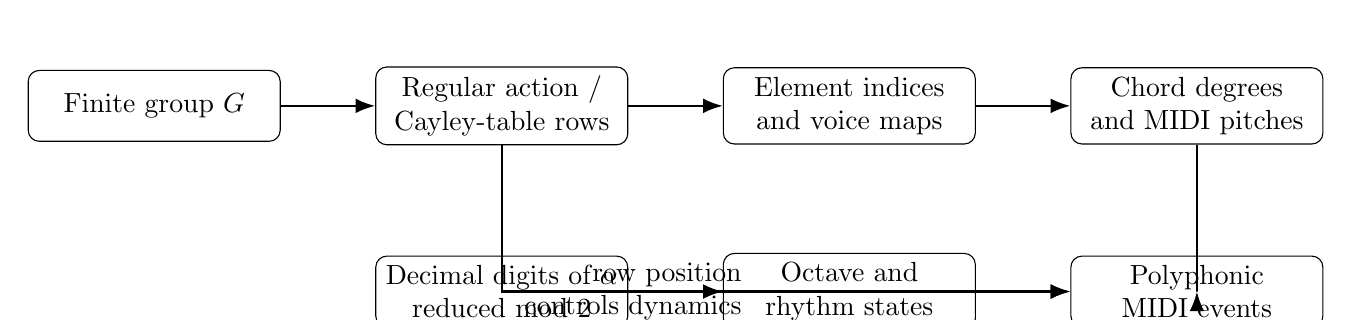
\begin{tikzpicture}[
    node distance=1.35cm and 1.2cm,
    box/.style={draw, rounded corners, align=center, minimum width=3.2cm, minimum height=0.9cm},
    arr/.style={-{Latex[length=2.5mm]}, thick}
]
\node[box] (group) {Finite group $G$};
\node[box, right=of group] (rows) {Regular action /\\Cayley-table rows};
\node[box, right=of rows] (index) {Element indices\\and voice maps};
\node[box, right=of index] (pitch) {Chord degrees\\and MIDI pitches};

\node[box, below=1.4cm of rows] (digits) {Decimal digits of $\alpha$\\reduced mod $2$};
\node[box, right=of digits] (state) {Octave and\\rhythm states};
\node[box, right=of state] (midi) {Polyphonic\\MIDI events};

\draw[arr] (group) -- (rows);
\draw[arr] (rows) -- (index);
\draw[arr] (index) -- (pitch);
\draw[arr] (digits) -- (state);
\draw[arr] (state) -- (midi);
\draw[arr] (pitch) |- (midi);
\draw[arr] (rows) |- node[pos=0.72,left,align=right]{row position\\controls dynamics} (midi);
\end{tikzpicture}%
}
\caption{Conceptual architecture of the composition system. Group structure controls pitch ordering, while an independent parity sequence controls register and rhythmic state.}
\end{figure}

\section{Interpretation: What Is Being Sonified?}

The procedure is best understood as a sonification of \emph{transformational structure}. A naive group sonification could assign one pitch to each element and play the elements in a fixed order. The present construction instead emphasizes the family of permutations generated by multiplication.

The most important invariant is that, for a genuine group enumeration without duplication, every Cayley-table row contains the same elements. What changes is their order. Musically, this means that the available symbolic material is conserved while its arrangement is transformed. This is closely aligned with the conceptual role of a group: the focus lies not only on objects, but on reversible transformations among them.

The harmonic and algebraic layers are deliberately separated. The chord list determines the harmonic language, while the group determines local ordering. Consequently, the same group can be rendered through very different harmonic vocabularies, and the same chord collection can be traversed by groups with different multiplication structures.

A useful summary is
\begin{center}
\fbox{\parbox{0.90\textwidth}{\centering The Cayley table of a finite group is read polyphonically through a harmonic coordinate system.}}
\end{center}

\section{Implementation Note on \texttt{iter\_it}}

The parameter \texttt{iter\_it} deserves a separate mathematical interpretation because its present behavior differs from what the word ``iteration'' might suggest.

Initially, the program sets
\[
n=|G|
\]
from the length of the original element list. If \texttt{iter\_it}>1, it then constructs a new list by repeatedly appending
\[
[g h : h\in G]
\]
for every $g$ in the original list. Since
\[
\{gh:h\in G\}=G
\]
for every $g\in G$, this operation creates repeated copies of the same group elements. For \texttt{iter\_it}=2, the new list has $n^2$ entries, but only $n$ distinct algebraic elements.

This has two consequences.

\subsection{Index overwriting}

The subsequent dictionary
\[
\texttt{idx}=\{g:i\}
\]
is constructed from a list containing duplicates. Each repeated group element overwrites its earlier dictionary entry, so the final index of an element corresponds to its last occurrence in the expanded list rather than to a canonical position in the original group enumeration.

Therefore the expanded index map no longer represents a one-to-one labeling of group elements by $0,\ldots,n-1$. The musical degree maps still function because indices are reduced modulo the current chord size, but their interpretation changes.

\subsection{Velocity saturation}

A second effect is subtler. The variable $n$ is computed \emph{before} the list expansion and is not updated afterwards. Hence the dynamic formulas continue to normalize by $n-1$, although the expanded orbit can contain $n^2$ positions. For sufficiently large $j$, the nominal even-voice velocity becomes strongly negative and is clipped to the MIDI minimum, while the odd-voice velocity becomes larger than 127 and is clipped to the MIDI maximum.

Thus \texttt{iter\_it}>1 currently produces a redundant multiset traversal together with increasing dynamic saturation. It is not, in its present form, an iterated regular representation, a Cartesian power $G^r$, a tensor product representation, or a higher-order group action.

This behavior may be musically useful as an intentional intensification mechanism, but it should be distinguished from genuine algebraic iteration.

\section{Possible Mathematical Extensions}

The present system already provides a coherent mapping from finite-group structure to music. Several extensions would preserve the same philosophy while strengthening the mathematical semantics.

\subsection{Canonical indexing under repetition}

If repeated passes through the group are desired, the canonical index map can remain attached to the original set $G$, while repetition is handled by a separate time index. This would preserve
\[
i:G\longrightarrow\{0,\ldots,n-1\}
\]
as a bijection.

\subsection{True iterated actions}

If a genuine higher-order construction is desired, one may let $G$ act diagonally on $G^r$:
\[
g\cdot(x_1,\ldots,x_r)
=
(gx_1,\ldots,gx_r).
\]
Alternatively, one may form direct products, semidirect products, or product actions and sonify the resulting orbit structures. Such constructions would give the iteration parameter a direct algebraic meaning.

\subsection{Conjugacy and class structure}

Another extension would replace or supplement the regular action with conjugation,
\[
x\longmapsto gxg^{-1}.
\]
This would organize musical material by conjugacy classes and could distinguish central elements from elements with larger conjugacy orbits.

\subsection{Representation-theoretic mappings}

A further development could use irreducible representations and character values. Instead of mapping element indices to chord degrees, one could derive pitch, timbre, density, or spatialization from matrix coefficients, traces, or character values. This would move the sonification from permutation structure toward the spectral structure of the group.

\section{Conclusion}

The composition system described in this paper transforms finite-group structure into polyphonic music through a sequence of explicit mappings. The regular action turns each group element into a permutation. Rows of the Cayley table become ordered paths. Group-element indices are projected onto degrees of a changing chord through several voice-dependent functions. A deterministic parity sequence derived from decimal digits controls reflected octave walks and cyclic redistribution of rhythmic values. Position inside each group-induced row controls dynamics.

The resulting music is therefore governed by several coupled but conceptually distinct mathematical layers. The group supplies symmetry and local ordering; the chord vocabulary supplies harmonic content; the digit-parity process supplies slower state changes; and MIDI realization turns these symbolic processes into sound.

The essential compositional principle can be stated compactly:
\begin{center}
\fbox{\parbox{0.88\textwidth}{\centering Preserve the material, transform its ordering, and let symmetry become musical motion.}}
\end{center}

\appendix
\section{Algorithmic Summary}

The following pseudocode summarizes the core musical process without reproducing details specific to the implementation.

\begin{lstlisting}[language=Python]
for g in group_elements:
    row = [g * h for h in group_elements]
    chord = choose_current_chord()
    bit = parity_digit[current_step]

    for position, x in enumerate(row):
        i = index[x]

        for voice in voices:
            degree = voice_map(voice, i, len(chord))
            pitch = chord[degree] + 12 * octave[voice]
            velocity = dynamic_profile(voice, position)
            duration = durations[voice]
            emit_midi_event(voice, pitch, duration, velocity)

    update_octaves(bit, previous_bit)

    if bit == 1:
        durations = rotate_left(durations)

    previous_bit = bit
\end{lstlisting}

\section{Executable Configuration Discussed Here}

The supplied implementation ultimately overwrites an earlier matrix-group example and uses the regular permutation representation of SageMath's \texttt{DihedralGroup(4)}. The active musical parameters are
\[
\text{tempo}=80,\qquad
\text{voices}=5,\qquad
D=\frac17,
\]
\[
\text{chord\_change\_every}=3,\qquad
\alpha=e^{-\pi},\qquad
\text{octave range}=[-2,2],
\]
with \texttt{iter\_it}=2 in the call to the music generator. The resulting event lists are written to a multi-track MIDI file.

\section*{Authorship Note}

Concept and code: Orges Leka.\\
Writing assistance and exposition: ChatGPT.

\end{document}
